\subsection{Architecture}

\begin{figure}[pht]
\begin{center}
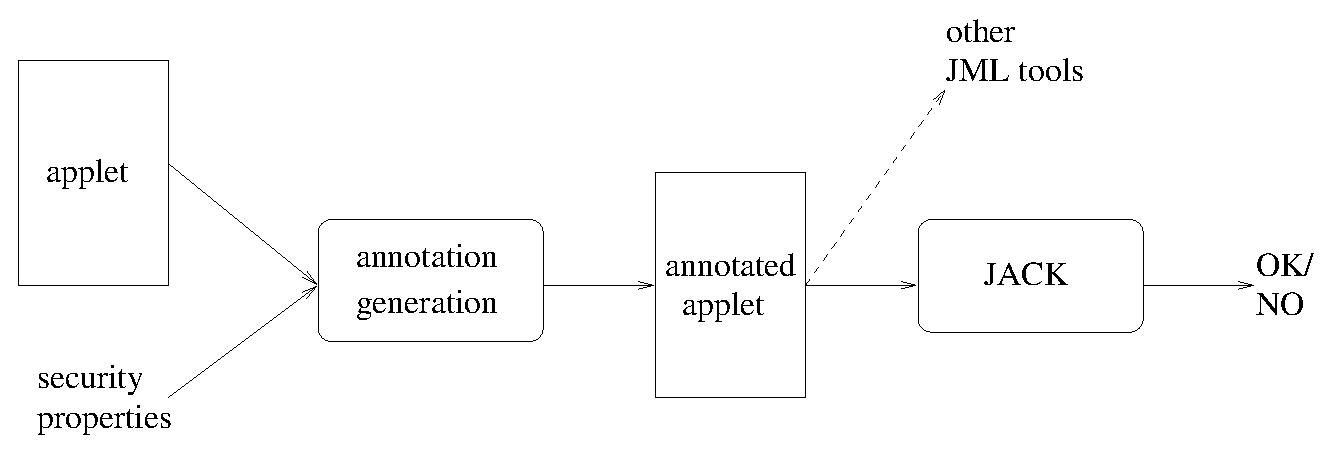
\epsfig{file=isaac/architecture.eps, width=9cm}
\end{center}
\caption{\sc Tool set for verifying high-level security properties}\label{FigArch}
\end{figure}



Figure~\ref{FigArch} shows the general architecture of the tool set
for verifying high-level security properties. Our annotation generator
can be used as a front-end for any tool accepting JML-annotated Java
(Card) applications. As input we have a security property and a Java
Card applet. The output is a JML Abstract Syntax Tree (AST), using the
format as defined for the standard JML parser. When pretty-printed,
this AST corresponds to a JML-annotated Java file. From this
annotated file, JACK generates appropriate proof obligations to check
whether the applet respects the security property.

\subsection{Automatic Generation of Annotations}

The propogation consists mainly on a weaving phase,
\emph{i.e.}~how the core-annotations are propagated throughout the
applet. We define functions \textsf{mod}, \textsf{pre}, \textsf{post} and
\textsf{exc\-post}, propagating assignable clauses, preconditions, 
postconditions and exceptional postconditions, respectively. These
functions have been defined and implemented for the full Java Card
language, but to present our ideas, we only give the definitions for a
representative subset of statements: statement composition, method
calls, conditional and \texttt{try}-\texttt{catch} statements and
special set-annotations. We assume the existence of domains
\textsf{MethName} of method names, \textsf{Stmt} of Java Card
statements, \textsf{Expr} of Java Card expressions, and \textsf{Var}
of static ghost variables, and functions
\textsf{call} and \textsf{body}, denoting a method call and 
body, respectively.

All functions are defined as mutual recursive functions on method
names, statements and expressions. When a method call is encountered,
the implementation will check whether annotations already have been
generated for this method (either by synthesizing or weaving). If not
it will recursively generate appropriate annotations. Java Card
applets typically do not contain (mutually) recursive method calls,
therefore this does not cause any problems. Generating appropriate
annotations for recursive methods would require more care (and in
general it might not be possible to do without any user interaction).

